% !TEX root = ../main.tex
\documentclass[../main.tex]{subfiles}

\begin{document}

\chapter{Role Fields: Mapping the Innovation Intermediary Field}
\labch{rolefield}
\margintoc

\begin{chapteroverview}
This chapter complements the inside-out perspective of the previous chapter with an outside-in approach. Rather than asking how KICs describe their relationships, we ask: how do external observers classify KICs and related actors? Using social curation methods, we map the European innovation intermediary field, identify sub-regions, and triangulate external classifications with internal role configurations.
\end{chapteroverview}

\begin{quote}
\textit{``Classifications are tools in strategies of inclusion and exclusion: whom to relate to and whom to isolate. They symbolize and consolidate patterns of inclusion and exclusion because they transform them into identities, which are taken for granted later on.''}\\
--- Wouter De Nooy \cite{denooy2003fields}
\end{quote}


%═══════════════════════════════════════════════════════════════════════════════
\section{Introduction: Opening the Field}[Introduction]
%═══════════════════════════════════════════════════════════════════════════════
\labsec{rolefield:intro}

\Cref{ch:interstitial} analyzed how KICs constitute their relational environments through self-presentation---an inside-out perspective. This chapter complements that view with an outside-in approach:\sidenote{\textbf{Triangulation}---combining inside-out and outside-in perspectives offers methodological triangulation on field structure.} How do external observers classify KICs and related actors? Who gets grouped together?

We leverage social curation mechanisms \sidecite{benabdelkrim-opening-fields-2020}---when users create lists grouping actors they perceive as related, their accumulated judgments reveal field structure \cite{bowker1999sorting,lazer2009computational}. This addresses conventional field study limitations: predetermined organizational forms, industry boundaries, and attribute-based rather than relational definitions.

The EIT ecosystem is ideal for this methodology. As interstitial organizations operating across the knowledge triangle, KICs span universities, corporations, startups, government agencies, and civil society. Curation-based mapping identifies who external observers perceive as belonging to the same relational space.

This chapter addresses three research questions:

\begin{enumerate}
    \item \textbf{CRQ1}: What is the structure of the European innovation intermediary field, and what sub-regions emerge?
    \item \textbf{CRQ2}: How are EIT KICs positioned---central, peripheral, or bridging?
    \item \textbf{CRQ3}: How do external classifications compare with organizational self-presentations?
\end{enumerate}


%═══════════════════════════════════════════════════════════════════════════════
\section{Methodology: Social Curation as Field Identification}[Social Curation]
%═══════════════════════════════════════════════════════════════════════════════
\labsec{rolefield:methods}

% ── Workflow Schematic ──────────────────────────────────────────────────────
\begin{wideblock}
\centering
\begin{tikzpicture}[
    scale=0.78, transform shape,
    stepbox/.style={draw, rounded corners=3pt, fill=#1!15,
        minimum width=2.6cm, minimum height=1.5cm,
        align=center, font=\scriptsize, inner sep=4pt},
    uibox/.style={draw, rounded corners=3pt, fill=CoverGold!25,
        minimum width=2.6cm, minimum height=1.5cm,
        align=center, font=\scriptsize, inner sep=4pt,
        line width=1pt},
    ethicslabel/.style={font=\fontsize{5.5}{6.5}\selectfont,
        text=AccentCoral!80!black, align=center, text width=2.4cm},
    arrow/.style={->, thick, PandaCharcoal!60},
]
    % ── Pipeline steps ──
    \node[stepbox=Azure] (s1) at (0,0)
        {\faUsers\\[0.15em]\textbf{Seed Selection}\\[0.1em]8 EIT accounts};
    \node[stepbox=AccentCyan] (s2) at (3.2,0)
        {\faList\\[0.15em]\textbf{Co-Classification}\\[0.1em]$k \geq 3$ threshold};
    \node[stepbox=AccentCyan] (s3) at (6.4,0)
        {\faProjectDiagram\\[0.15em]\textbf{Network Expansion}\\[0.1em]12,847 actors};
    \node[stepbox=AccentPurple] (s4) at (9.6,0)
        {\faSitemap\\[0.15em]\textbf{Community Detection}\\[0.1em]Louvain, 10 regions};
    \node[stepbox=PandaBamboo] (s5) at (12.8,0)
        {\faRetweet\\[0.15em]\textbf{Mention Network}\\[0.1em]268,309 tweets};
    \node[uibox] (ui) at (16,0)
        {\faDesktop\\[0.15em]\textbf{ROLEFIELD}\\[0.1em]Interactive UI};

    % ── Arrows ──
    \draw[arrow] (s1) -- (s2);
    \draw[arrow] (s2) -- (s3);
    \draw[arrow] (s3) -- (s4);
    \draw[arrow] (s4) -- (s5);
    \draw[arrow] (s5) -- (ui);

    % ── Ethics annotations ──
    \node[ethicslabel] at (0,-1.3)
        {\faBalanceScale~Seed bias:\\institutional accounts};
    \node[ethicslabel] at (3.2,-1.3)
        {\faBalanceScale~Pre-2023 API:\\terms of service};
    \node[ethicslabel] at (6.4,-1.3)
        {\faBalanceScale~Account privacy:\\public profiles only};
    \node[ethicslabel] at (9.6,-1.3)
        {\faBalanceScale~Algorithm sensitivity:\\resolution parameter};
    \node[ethicslabel] at (12.8,-1.3)
        {\faBalanceScale~Temporal snapshot:\\data not reproducible};
    \node[ethicslabel] at (16,-1.3)
        {\faLockOpen~Open source:\\full transparency};
\end{tikzpicture}
\captionof{figure}{Analytical workflow for field mapping through social curation. Ethical considerations (coral) annotate each step. The pipeline flows from seed selection through co-classification network construction, community detection, and triangulation with mention networks. The \textsc{Rolefield} UI enables interactive exploration.}
\label{fig:ch6:workflow}
\end{wideblock}

\subsection{Co-Classification Logic}

When Twitter users create lists grouping accounts they perceive as related, repeated co-classification by independent curators reveals relational proximity.\sidenote{\textbf{Social curation}---accumulating classification acts collectively reveal who belongs together.} Two actors $a_i$ and $a_j$ are connected if jointly classified in $\geq k$ lists (default: $k = 3$). This captures external perceptions through symmetric, observer-made classifications requiring third-party validation.

We implement \textcite{benabdelkrim-opening-fields-2020}'s procedure: (1) select seed accounts, (2) discover two-ring networks via list co-memberships, (3) denoise through random walk centrality, (4) merge seed networks, (5) visualize with force-directed layout, (6) detect communities.\sidenote{\textbf{Iterative expansion}---enables field discovery without predetermined boundaries.} Sub-regions are identified using the Louvain algorithm \cite{blondel2008louvain}, which groups actors more densely connected internally than externally. Twitter biography content analysis (TF-IDF weighted n-grams) characterizes each sub-region. The ten-region structure is stable across parameter variations ($k \in \{2,3,4\}$; resolution $\in \{0.5,1.0,1.5\}$).


%═══════════════════════════════════════════════════════════════════════════════
\section{Data Collection: Seeding the EIT Field}[Data Collection]
%═══════════════════════════════════════════════════════════════════════════════
\labsec{rolefield:data}

We selected eight seed accounts spanning the EIT ecosystem:\sidenote{\textbf{Seed selection}---captures institutional core while varying by domain and maturity.} @EIT\_EU (institutional), @ClimateKIC, @EITDigital, @InnoEnergy (established KICs), @EITHealth, @EITFood, @EIT\_Urban (newer KICs), and @EITCommunity (cross-cutting). Data collection via Twitter API (pre-2023 restrictions) included user profiles, list memberships, and tweet mentions via TweetBinder.\sidenote{\textbf{TweetBinder}---structured exports of tweet data including mentions and engagement.} Parameters: $k = 3$ co-classification threshold, max 100 lists per user, two-ring expansion (10,000/100,000 user limits).


%═══════════════════════════════════════════════════════════════════════════════
\section{Findings: Structure of the Innovation Intermediary Field}[Field Structure]
%═══════════════════════════════════════════════════════════════════════════════
\labsec{rolefield:findings}

\subsection{Aggregate Network Properties}

Merging the eight seed networks produced a connected network of actors linked by co-classification relations.\sidenote{\textbf{Connectedness}---the network's connectedness confirms that seeds belong to a coherent relational space, not isolated sub-fields.} Table \ref{tab:rolefield:coclassification-stats} summarizes the key properties of the co-classification network.

\begin{center}
\small
\begin{tabular}{lrl}
\toprule
\textbf{Property} & \textbf{Value} & \textbf{Interpretation} \\
\midrule
Actors & 12,847 & Field participants (co-classified) \\
Co-classification edges & 487,293 & Undirected similarity ties \\
Density & 0.006 & Selective connection \\
Modularity & 0.72 & Clear community structure \\
Components & 1 (main) & Unified relational space \\
Sub-regions & 10 & Louvain communities \\
\bottomrule
\end{tabular}
\captionof{table}{Co-Classification Network Statistics}
\labtab{rolefield:coclassification-stats}
\end{center}

The single connected component confirms that all seeds---despite spanning different thematic domains---are perceived by external curators as belonging to a unified relational space.


\subsection{Ten Sub-Regions}

Louvain detection identified ten sub-regions:\sidenote{\textbf{ForceAtlas2}---visualization layout where connected actors attract, unconnected repel.} Climate \& Sustainability, Digital \& Tech Startups, Health Innovation, EU Policy \& Funding, Higher Education, Impact \& Social Innovation, Food \& Agriculture, Urban \& Mobility, Venture Capital, and Corporate Innovation. Twitter biography content analysis (TF-IDF weighted terms) characterizes each. Manual coding of 200 random actors reveals substantial heterogeneity: individuals (33\%), startups (22\%), research institutions (12\%), universities (11\%), corporations (8\%), government (6\%), NGOs (4\%), media (3\%), and associations (1\%). No single organizational form dominates---the field is constituted by relations among diverse actors.

KICs exhibit \textit{thematic anchoring}: each sits near its thematic sub-region center (EIT Health near Health Innovation, EIT Food near Food \& Agriculture). They also perform \textit{cross-regional bridging}, maintaining connections to EU Policy \& Funding and Higher Education. The EIT institutional account occupies a central position across all sub-regions.


%═══════════════════════════════════════════════════════════════════════════════
\section{Triangulation: External Classification Meets Internal Configuration}[Triangulation]
%═══════════════════════════════════════════════════════════════════════════════
\labsec{rolefield:triangulation}

\Cref{ch:interstitial} identified sociotype configurations from self-presentations; this chapter identifies field structure from external classifications. How do these align?\sidenote{\textbf{Validity check}---tests whether organizational self-understanding corresponds to external perception.}

The five sociotypes map onto external sub-regions: Connective (distributed across regions, not localized---connection is a \textit{function}, not a domain), Acceleration (Venture Capital; Digital \& Tech), Development (Higher Education), Knowledge (research institutions), and Accountability (EU Policy \& Funding). Domain contexts (not sociotypes) correspond to thematic communities (Climate, Health, Food), validating internal sectoral positioning. The peripheral Accountability sociotype corresponds to a distinct external EU Policy sub-region, confirming that accountability relationships form a coherent relational space.

Bridging actors (high cross-sub-region connections) include umbrella organizations (EIT, European Commission), broad-coverage media, multi-domain individuals, and cross-sectoral funders. KICs exhibit an \textbf{interfacing} pattern: classified with thematic peers but maintaining substantial cross-regional connections.\sidenote{\textbf{Interface pattern}---balanced within/across-region ratios validate multivocal category exploitation.}


%═══════════════════════════════════════════════════════════════════════════════
\section{Discussion: What External Classification Reveals}[Discussion]
%═══════════════════════════════════════════════════════════════════════════════
\labsec{rolefield:discussion}

The curation-based approach reveals three key patterns.\sidenote{\textbf{Perception vs.\ reality}---captures the field as it exists in collective perception.} First, \textbf{thematic organization}: the field is organized by sector (climate, health, digital) rather than organizational type or geography. External observers perceive KICs' knowledge triangle integration through sectoral lenses. Second, \textbf{EU policy as distinct region}: the public accountability dimension---peripheral in KIC self-presentation---is recognized externally as a coherent relational space. Third, \textbf{individual prominence}: 33\% of actors are individuals (professionals, entrepreneurs, researchers), underscoring that fields are constituted by persons inhabiting institutions.

Limitations include curator bias (Twitter list creators reflect particular vantage points), platform specificity (actors absent from Twitter are invisible), temporal snapshot effects, and semantic ambiguity (co-classification doesn't reveal \textit{why} actors are grouped). Triangulation with internal perspectives is essential: alignment builds confidence, divergence reveals gaps between perception and self-understanding. The methodology captures actor heterogeneity without organizational form restrictions and enables tracking field evolution as KICs mature.


%═══════════════════════════════════════════════════════════════════════════════
\section{Interim Summary: Co-Classification Findings}[Co-Classification Summary]
%═══════════════════════════════════════════════════════════════════════════════
\labsec{rolefield:interim}

Co-classification analysis mapped the European innovation intermediary field through social curation. Key findings: (1) ten thematic sub-regions, (2) KICs anchor sub-regions while bridging the broader ecosystem, (3) substantial actor heterogeneity, (4) EU policy as distinct sub-region validating internal accountability configuration.\sidenote{\textbf{External validation}---strengthens claims about KICs' distinctive character.} We now turn to Twitter mention networks, which capture \textit{performed} engagement rather than \textit{perceived} similarity.


%═══════════════════════════════════════════════════════════════════════════════
\section{Empirical Analysis: Twitter Mention Networks}[Twitter Networks]
%═══════════════════════════════════════════════════════════════════════════════
\labsec{rolefield:empirical}

We analyze 268,309 tweets from the EIT ecosystem (January 2015--August 2020) mentioning seed account handles.\sidenote{\textbf{Data source}: TweetBinder exports with EIT KIC mentions and hashtags.} This mention network captures \textit{performed} engagement---who actually engages with whom---complementing the \textit{perceived} similarity from co-classification.

\subsection{Network Construction}

From the tweet corpus, we extract mention edges (actor A mentioned actor B) and retweet edges (actor A amplified actor B's content). Applying a minimum threshold of 3 interactions yields a mention network with the properties shown in Table \ref{tab:rolefield:network-stats}.

\begin{center}
\small
\begin{tabular}{lrl}
\toprule
\textbf{Property} & \textbf{Value} & \textbf{Interpretation} \\
\midrule
Actors & 65,046 & Field participants \\
Mention edges & 73,879 & Directed engagement ties \\
Density & 0.00002 & Highly selective engagement \\
Modularity & 0.64 & Strong community structure \\
Components & 38,253 & Fragmented periphery \\
Largest component & 40.5\% & Core-periphery structure \\
Communities & 96 & Louvain communities \\
\bottomrule
\end{tabular}
\captionof{table}{Mention Network Statistics (2015--2020)}
\labtab{rolefield:network-stats}
\end{center}

The high modularity (0.64) confirms strong community structure---actors cluster around shared engagement patterns.\marginnote{The 96 communities detected are dominated by 8 major communities corresponding to KIC thematic domains.} The core-periphery structure (largest component containing only 40.5\% of actors) reflects the field's combination of densely connected institutional cores surrounded by loosely connected peripheral actors.

Figure \ref{fig:rolefield:network} visualizes the mention network, with nodes colored by community membership and sized by degree centrality. The network reveals the characteristic structure of the EIT ecosystem: distinct KIC-centered clusters connected through bridging actors and cross-cutting thematic nodes.

\begin{center}
\includegraphics[width=\textwidth]{figures/rolefield-network.pdf}
\captionof{figure}{EIT Twitter mention network (top 200 actors by degree). Node colors indicate community membership; node size reflects degree centrality. KIC accounts anchor distinct communities while maintaining cross-community connections.}
\label{fig:rolefield:network}
\end{center}

\subsection{Attention Hierarchy: Most Mentioned Accounts}

Table \ref{tab:rolefield:top-mentioned} presents the most mentioned accounts, revealing the attention hierarchy of the EIT ecosystem.

\begin{center}
\small
\begin{tabular}{lrrl}
\toprule
\textbf{Account} & \textbf{Mentions} & \textbf{Share} & \textbf{KIC Affiliation} \\
\midrule
@ClimateKIC & 104,759 & 39.1\% & Climate-KIC \\
@EITeu & 50,294 & 18.8\% & EIT Central \\
@EIT\_Digital & 39,354 & 14.7\% & EIT Digital \\
@CKICNordic & 19,723 & 7.4\% & Climate-KIC \\
@EITRawMaterials & 19,346 & 7.2\% & EIT RawMaterials \\
@InnoEnergyEU & 12,909 & 4.8\% & InnoEnergy \\
@EITDigitalAccel & 9,970 & 3.7\% & EIT Digital \\
@EUeic & 9,603 & 3.6\% & EU Policy \\
@EITHealth & 4,022 & 1.5\% & EIT Health \\
@EITUrbanMob & 3,592 & 1.3\% & EIT Urban Mobility \\
\bottomrule
\end{tabular}
\captionof{table}{Top 10 Most Mentioned Accounts}
\labtab{rolefield:top-mentioned}
\end{center}

\begin{insightbox}[Climate-KIC Dominance]
Climate-KIC accounts for 39\% of all mentions---nearly double the EIT central account (19\%). This dominance reflects Climate-KIC's status as an original 2010 KIC, its broad thematic scope (climate intersects all sectors), and its particularly active social media presence.
\end{insightbox}

\subsection{KIC Subnetworks and Attention Hierarchy}

KIC subnetworks vary in size and density:\sidenote{Density inversely correlates with size---smaller KICs maintain tighter networks.} Climate-KIC (9,824 actors, density 0.00025) is 2.5$\times$ larger than EIT Digital (3,998 actors, 0.00063), reflecting thematic breadth. EIT RawMaterials shows highest density (0.00112) despite smaller size (1,935 actors), suggesting a tight-knit specialist community. Climate-KIC dominates the attention hierarchy with 39\% of all mentions (104,759), nearly double the EIT central account (50,294, 19\%). \Cref{fig:rolefield:mention-dist} shows the mention distribution.

% Figure: Mention Distribution
\begin{center}
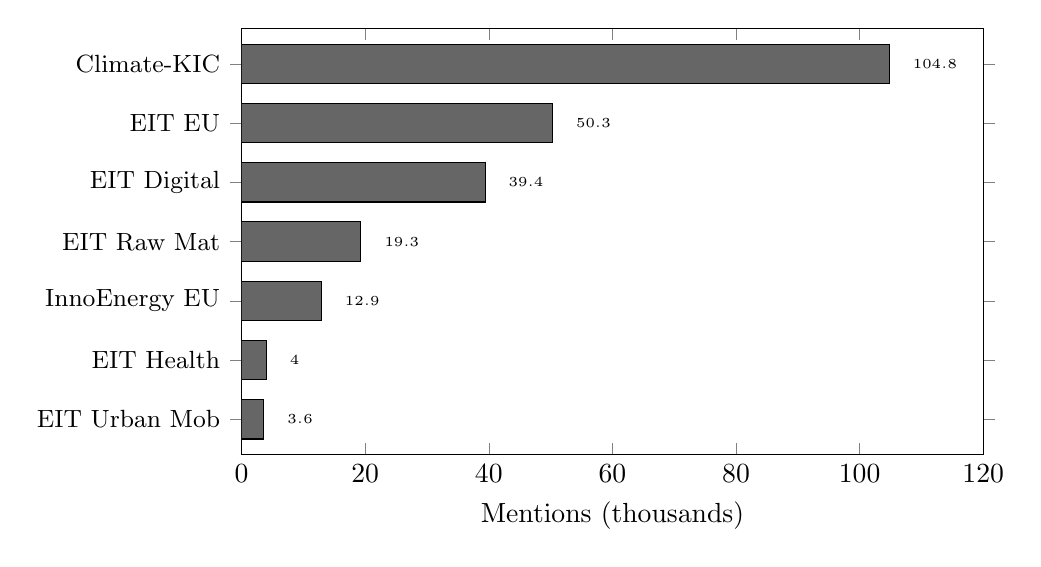
\begin{tikzpicture}
\begin{axis}[
    xbar,
    width=11cm,
    height=7cm,
    xlabel={Mentions (thousands)},
    symbolic y coords={
        EIT Urban Mob,
        EIT Health,
        InnoEnergy EU,
        EIT Raw Mat,
        EIT Digital,
        EIT EU,
        Climate-KIC
    },
    ytick=data,
    y tick label style={font=\small},
    xmin=0,
    xmax=120,
    bar width=0.5cm,
    nodes near coords,
    nodes near coords style={font=\tiny},
    every node near coord/.append style={xshift=5pt},
]
\addplot[xbar, fill=black!60] coordinates {
    (104.8,Climate-KIC)
    (50.3,EIT EU)
    (39.4,EIT Digital)
    (19.3,EIT Raw Mat)
    (12.9,InnoEnergy EU)
    (4.0,EIT Health)
    (3.6,EIT Urban Mob)
};
\end{axis}
\end{tikzpicture}
\captionof{figure}{Mention distribution across top EIT accounts}
\labfig{rolefield:mention-dist}
\end{center}

\subsection{Bridging Actors}

High-bridging actors (cross-community connections) include thematic connectors (circular economy, climate) and amplification accounts that redistribute content across communities.\sidenote{\textbf{Bridging score}: Proportion of ties crossing community boundaries.} This validates the theoretical expectation that bridging is performed by actors at categorical intersections.

\subsection{Temporal Dynamics}

Tweet volume grew from 24,300 (2015) to a peak of 64,600 (2018), then declined to 33,400 (2020).\marginnote{2020 decline reflects COVID-19 disruption and data collection ending in August.} This trajectory corresponds to ecosystem maturation as newer KICs (EIT Health 2015, EIT Food 2017, EIT Urban Mobility 2018) joined the Twitter conversation.

\subsection{Triangulation: Mentions vs.\ Classification}

Internal sociotypes align with external engagement patterns: Connective (high bridging scores), Acceleration (EIT Digital density), Development (Higher Ed presence), Knowledge (research mentions), Accountability (EU Policy mentions), and Sectoral (subnetwork separation).\marginnote{Key validation: ecosystem orchestration is \textit{performed} through cross-community engagement, not merely claimed.} Actor heterogeneity (33\% individuals, 22\% startups, 12\% research, 11\% universities) confirms fields are constituted by diverse actor types.


\subsection{Phase-Out Roles: The Relational Gap}

The relational field is entirely oriented toward build-up dynamics.\sidenote{\textbf{Build-up field}---social curation and engagement cluster around innovation, not destabilization.} All ten sub-regions represent \emph{new value creation}. No sub-region focuses on managed decline, fossil fuel phase-out, or carbon-intensive industry wind-down. No bridging actors connect sunset sectors with transition support. Twitter engagement verbs (\emph{supports}, \emph{launches}, \emph{accelerates}) describe build-up; no discourse clusters around \emph{divestment}, \emph{decommissioning}, or \emph{just transition}. The absence of phase-out patterns in \emph{enacted} social relations---not just claimed identities---suggests the gap is substantive, not merely rhetorical.

%═══════════════════════════════════════════════════════════════════════════════
\section{Chapter Summary}
%═══════════════════════════════════════════════════════════════════════════════

\textbf{CRQ1: Field structure.} Co-classification reveals a unified field organized into ten thematic sub-regions (Climate \& Sustainability, Digital \& Tech, Health, EU Policy, Higher Education, Impact, Food, Urban, Venture Capital, Corporate Innovation). Modularity (0.72 for co-classification, 0.64 for mentions) indicates clear community structure. Twitter mention network (268,309 tweets, 65,046 actors) confirms this with 96 communities.

\textbf{CRQ2: KIC positioning.} KICs exhibit \textit{interfacing}: anchoring thematic sub-regions while maintaining cross-regional connections. Climate-KIC dominates attention (39\% of mentions) reflecting thematic breadth. Subnetworks vary: Climate-KIC largest (9,824 actors), RawMaterials most cohesive (density 0.00112). Density inversely correlates with size.

\textbf{CRQ3: Internal-external alignment.} Triangulation reveals strong alignment: five sociotypes (Connective, Acceleration, Development, Knowledge, Accountability) map onto external sub-regions and engagement patterns. Connective validated through high bridging scores. Accountability corresponds to EU Policy sub-region. Phase-out roles absent from both claimed identities and enacted relations---substantive gap, not rhetorical.

\begin{summarybox}
\begin{itemize}[leftmargin=*, itemsep=0.3em]
\item \textbf{Social curation} maps field structure without predetermined boundaries via external classification acts.
\item \textbf{Ten sub-regions} organized thematically, not by organizational type or geography.
\item \textbf{Climate-KIC dominance}: 39\% of mentions, reflecting scale and social media activity.
\item \textbf{KIC interfacing}: anchor thematic domains while bridging cross-regionally.
\item \textbf{Triangulation} validates Connective roles performed through cross-community bridging.
\item \textbf{Breakdown gap}: No relational clustering around managed decline or phase-out---substantive absence.
\end{itemize}
\end{summarybox}

\vspace{0.5em}
\begin{replicationbox}[Data \& Code Availability]
\texttt{rolebox-social} module: \texttt{src/rolebox\_social/}, \texttt{notebooks/field\_mapping\_demo.ipynb}, \texttt{ui/rolefield.html} (interactive visualization), \texttt{data/outputs/field\_analysis.json}. Raw data: 268,309 tweets (2015--2020).
\end{replicationbox}

\vspace{1em}
The next chapter examines portfolio compositions through venture data.\sidenote{\textit{Next}: \textbf{\Cref{ch:venture}}---Venture Positioning analyzes EIT portfolio compositions.}

\end{document}
